\documentclass{exam}
\usepackage[utf8]{inputenc}
\usepackage{lmodern}
\usepackage{microtype}

% \usepackage[parfill]{parskip}
\usepackage[dvipsnames]{xcolor}
\usepackage{amsmath}
\usepackage{amsfonts}
\usepackage{amsthm}
\usepackage{siunitx}
\DeclareSIUnit\year{yr}
\DeclareSIUnit\foot{ft}
\DeclareSIUnit\litre{\liter}

\usepackage{skull}

\usepackage{pgfplots}
\usepgfplotslibrary{polar}
\pgfplotsset{compat=1.11}
\usepgfplotslibrary{statistics}
\usepackage{graphicx}
\usepackage{sidecap}
\sidecaptionvpos{figure}{c}
\usepackage{float}
\usepackage{gensymb}
\usepackage{tkz-euclide}
\usetkzobj{all}
\usepackage{commath}
\usepackage{hyperref}
\usepackage{enumitem}
\usepackage{wasysym}
\usepackage{multicol}
\usepackage{mathtools}
\usepackage{tcolorbox}
\usepackage{tabularx}
\usepackage[version=4]{mhchem}
\usepackage{changepage}
\usepackage{listings}
\lstset{basicstyle=\ttfamily\linespread{0.8}\small}

\renewcommand*{\thefootnote}{\fnsymbol{footnote}}

\newtheorem*{thm}{Theorem}
\newtheorem*{iden}{Identity}
\newtheorem*{lemma}{Lemma}
\newtheorem{obs}{Observation}
\theoremstyle{definition}
\newtheorem*{defn}{Definition}
\newtheorem*{ex}{Example}
\newtheorem{con}{Construction}
\newtheorem*{alg}{Algorithm}

\newtheoremstyle{break}
  {\topsep}{\topsep}%
  {\itshape}{}%
  {\bfseries}{}%
  {\newline}{}%
\theoremstyle{break}
\newtheorem*{bthm}{Theorem}

% russian integral
\usepackage{scalerel}
\DeclareMathOperator*{\rint}{\scalerel*{\rotatebox{17}{$\!\int\!$}}{\int}}

% \DeclareMathOperator*{\rint}{\int}

\pgfplotsset{vasymptote/.style={
    before end axis/.append code={
        \draw[densely dashed] ({rel axis cs:0,0} -| {axis cs:#1,0})
        -- ({rel axis cs:0,1} -| {axis cs:#1,0});
    }
}}

% \pointsinrightmargin
\boxedpoints
\pointname{}

\newcommand{\questioA}{\question[\texttt{\textbf{\color{Cerulean} A}}]}
\newcommand{\questioM}{\question[\texttt{\textbf{\color{PineGreen} M}}]}
\newcommand{\questioE}{\question[\texttt{\textbf{\color{WildStrawberry} E}}]}
\newcommand{\questioS}{\question[\texttt{\textbf{\color{Goldenrod} S}}]}
\newcommand{\questioO}{\question[\texttt{\textbf{\color{BurntOrange} O}}]}

\newcommand{\parA}{\part[\texttt{\textbf{\color{Cerulean} A}}]}
\newcommand{\parM}{\part[\texttt{\textbf{\color{PineGreen} M}}]}
\newcommand{\parE}{\part[\texttt{\textbf{\color{WildStrawberry} E}}]}
\newcommand{\parS}{\part[\texttt{\textbf{\color{Goldenrod} S}}]}
\newcommand{\parO}{\part[\texttt{\textbf{\color{BurntOrange} O}}]}

\newcommand{\subparA}{\subpart[\texttt{\textbf{\color{Cerulean} A}}]}
\newcommand{\subparM}{\subpart[\texttt{\textbf{\color{PineGreen} M}}]}
\newcommand{\subparE}{\subpart[\texttt{\textbf{\color{WildStrawberry} E}}]}
\newcommand{\subparS}{\subpart[\texttt{\textbf{\color{Goldenrod} S}}]}
\newcommand{\subparO}{\subpart[\texttt{\textbf{\color{BurntOrange} O}}]}

\newcommand{\mainHeader}[2]{\section*{NCEA Level 2 Mathematics\\#1. #2}}
\newcommand{\mainHeaderHw}[2]{\section*{NCEA Level 2 Mathematics (Homework)\\#1. #2}}
\newcommand{\seealso}[1]{\begin{center}\emph{See also #1.}\end{center}}
\newcommand{\drills}[1]{\begin{center}\emph{Drill problems: #1.}\end{center}}
\newcommand{\basedon}[1]{\begin{center}\emph{Notes largely based on #1.}\end{center}}


\begin{document}

\mainHeader{16}{Counting and Combinatorics}
We move from calculus, the study of the continuous, to combinatorics, the study of the discrete. We begin with a simple
question: how many ways are there of picking a committee of three people, given a group of six people? Our first attempt
at this is relatively naive: there are six choices for the first person in the committee, five for the second, and four
for the third --- so $ 6 \times 5 \times 4 = 120 $ altogether. The problem with this is that we have overcounted: suppose
our six people are labelled from $ A $ to $ F $; then we have (for example) counted $ ABC $ and $ BAC $ separately (because
in one we picked $ A $ first, and in the other we picked $ B $ first) despite the simple fact that they are the same committee!

In order to solve this problem, we need to count cleverer. Because the solution in this case works in general, we'll work it
out in general to save time. So suppose we have a group of $ n $ people, and we want to pick a committee of $ r $ of them. Then,
if we count different orderings separately, we obtain
\begin{displaymath}
  n(n-1)\cdots(n - r + 1) = \frac{n!}{(n - r)!}
\end{displaymath}
different committees (where the notation $ n! $, read $ n $ bang or $ n $ factorial, denotes $ n(n-1)\cdots3 \cdot 2 \cdot 1 $). This
is the problem we solved above (and is called the number of permutations of $ r $ things out of $ n $ in total, or $ {}^nP_r $); we just
need to divide through by the number of times we counted each group. There are $ r! $ different orderings for a set of $ r $ people, and
so we counted each committee of $ r $ people $ r! $ times in total --- once for each ordering. Hence the total number of committees
possible, up to ordering, is
\begin{displaymath}
  \frac{n!}{(n - r)!r!} = \binom{n}{r} = {}^nC_r
\end{displaymath}
which is read `$ n $ choose $ r $'. We have therefore proved:

\begin{thm}
  The number of ways to choose $ r $ objects from a set of $ n $, if we don't care about order, is
  given by $ \binom{n}{r} $. If we care about order, the number of choices for the smaller set
  is given by $ {}^nP_r $.
\end{thm}

There is an interesting pattern that we can make with these `choice constants', known as \emph{Pascal's triangle} after
French mathematician Blaise Pascal.
\begin{gather*}
  1\\
  1 \quad 1\\
  1 \quad 2 \quad 1\\
  1 \quad 3 \quad 3 \quad 1\\
  1 \quad 4 \quad 6 \quad 4 \quad 1\\
  1 \quad 5 \quad 10 \quad 10 \quad 5 \quad 1\\
  \cdots
\end{gather*}
The row number (starting from zero) is $ n $, and the column number (from the left and starting from zero) is $ r $. Let's look at some of the patterns here.
\begin{obs}
  The first and last column of each row is 1. In our counting notation, this is the observation that $ \binom{n}{0} = \binom{n}{n} = 1 $
  for all sets of size $ n $.
\end{obs}
\begin{proof}
  We need to check that each observation is true for the whole table, not just the portion I gave above. This proof is left
  to you!
\end{proof}

\begin{obs}
  The second and $ r - 1$th column of each row is just $ n $ (except the first). In our counting notation, this is the observation
  that $ \binom{n}{1} = \binom{n}{n - 1} = n $.
\end{obs}
\begin{proof}
  We need to check that each observation is true for the whole table, not just the portion I gave above. This proof is left
  to you! This one can be done either by using the factorial formula, or by counting.
\end{proof}

\begin{obs}
  The triangle is symmetric about the middle axis. In our counting notation, this is the observation that $ \binom{n}{r} = \binom{n}{n - r} $.
\end{obs}
\begin{proof}[Proof 1: less satisfying]
  \begin{displaymath}
    \binom{n}{r} = \frac{n!}{(n - r)!r!} = \frac{n!}{r!(n - r)!} = \binom{n}{n - r}
  \end{displaymath}
\end{proof}
\begin{proof}[Proof 2: counting]
  Suppose we pick a subset of size $ r $ out of our set of size $ n $. This also uniquely identifies
  a subset of size $ n - r $: the elements we didn't take! Since there is a one-to-one correspondence
  between picking sets of size $ r $ and sets of size $ n - r $, the number of choices for both sizes
  of subset must be the same.
\end{proof}

\begin{obs}
  Each number is given by the sum of the two numbers diagonally above from it. In our counting notation, this is the observation
  that $ \binom{n - 1}{r - 1} + \binom{n - 1}{r} = \binom{n}{r} $.
\end{obs}
\begin{proof}
  Pick some object $ x $ in our larger set of size $ n $. Then we are left with some set of size $ n - 1 $ left over. If we want to pick
  a subset of size $ r $ from the set of size $ n $, then we have two cases: either the subset we pick contains $ x $, or it does not. If
  it contains $ x $, we need to pick another $ r - 1 $ things from the remaining $ n - 1 $ in order to fill our set up; if it does not,
  then we need to pick up a full $ r $ things from the remaining $ n - 1 $. In the first case, there are $ \binom{n - 1}{r - 1} $ choices;
  in the second case, there are $ \binom{n - 1}{r} $ choices.
\end{proof}


\begin{obs}
  The sum of all the numbers in a row is $ 2^n $:
  \begin{gather*}
    2^0 = 1\\
    2^1 = 1 + 1\\
    2^2 = 1 + 2 + 1\\
    2^3 = 1 + 3 + 3 + 1\\
    2^4 = 1 + 4 + 6 + 4 + 1\\
    2^5 = 1 + 5 + 10 + 10 + 5 + 1\\
  \end{gather*}
\end{obs}
\begin{proof}
  The sum of all the numbers in a row is the total number of ways we can choose subsets of size zero, plus subsets
  of size one, all the way up to subsets of size $ n $: in short, the sum is just the total number of subsets of the
  larger set. But there are $ 2^n $ different subsets of the larger set (for each element, we either keep it or not: $ n $ choices,
  with two possible outcomes for each).
\end{proof}

I will only give one application of Pascal's triangle and the counting numbers here, but rest assured there are many others.

\begin{ex}
  Recognise this pattern?
  \begin{enumerate}
    \item $ (x + y)^1 = {\bf\color{red}1}x + {\bf\color{red}1}y $
    \item $ (x + y)^2 = {\bf\color{red}1}x^2 + {\bf\color{red}2}xy + {\bf\color{red}1}y^2 $
    \item $ (x + y)^3 = {\bf\color{red}1}x^3 + {\bf\color{red}3}x^2y + {\bf\color{red}3}xy^2 + {\bf\color{red}1}y^3 $
    \item $ (x + y)^4 = {\bf\color{red}1}x^4 + {\bf\color{red}4}x^3 y + {\bf\color{red}6}x^2 y^2 + {\bf\color{red}4}x y^3 + {\bf\color{red}1}y^4 $
  \end{enumerate}
\end{ex}

\begin{thm}[Binomial theorem]
  \begin{displaymath}
    (x + y)^n = \binom{n}{0} x^n y^0 + \binom{n}{1} x^{n - 1} y^1 + \cdots + \binom{n}{r} x^{n - r} y^r + \cdots + \binom{n}{n - 1} x^1 y^{n - 1} + \binom{n}{n} x^0 y^n
  \end{displaymath}
\end{thm}
\begin{proof}
  Recall how expanding binomials work: we write
  \begin{displaymath}
    (x + y)^n = (x + y)(x + y)\cdots(x + y)
  \end{displaymath}
  and then expand using the distributive law. Each term in the result consists of either $ x $ or $ y $ from the first bracket,
  either $ x $ or $ y $ from the second, and so on until we pick either $ x $ or $ y $ from the final bracket; so each term contains
  exactly $ n $ $ x$'s and $ y$'s, and there is one term for each possible combination of picking things from brackets. In fact,
  there will be $ \binom{n}{r} $ terms with $ r $ $ x$'s --- because that is the number of different ways to pick $ r $ $ x$'s out
  of the $ n $ brackets. The remaining $ n - r $ things we picked for each of those terms must be $ y$'s; and we when we add up the
  terms where we pick 0 $ x$'s, 1 $ x $, 2 $ x$'s, and so on, we obtain the desired result.
\end{proof}

Because of this proof, the counting coefficients $ \binom{n}{r} $ are more properly called \emph{binomial coefficients}.

\subsection*{Questions}
\begin{questions}
  \question Given that $ n! $ is the number of orderings of $ n $ objects, explain why $ 0! = 1 $ is a reasonable definition.
  \question I have a bucket of 10 numbered balls, and a bucket of 10 green balls that all look the same.
    \begin{parts}
      \part Suppose I pick a set of five balls from each. How many different ways are there of doing this if I count two sets the same when
            I can't tell them apart?
      \part How many different ways are there of picking a set of ten balls, but this time I pick randomly from both buckets?
    \end{parts}
  \question How many words of exactly ten characters are possible with an alphabet of 26 characters if:
    \begin{parts}
      \part Repetitions are allowed.
      \part Repetitions are not allowed at all.
      \part Repetitions are allowed, but adjacent characters must be different.
    \end{parts}
  \question Repeat question 3, but now for words of ten characters or less.
  \question Verify the binomial theorem for $ (2 + 3)^4 $, by both doing the exponent and by expanding out. (This allows us to
            split a large exponential operation into several smaller ones.)
  \question
    \begin{parts}
      \part Add up $ 1 + 2 + \cdots + 99 + 100 $.
      \part Add up $ 1 + 2 + \cdots + (n - 1) + n $. How many different proofs of the resulting formula can you think of? Hint:
            \begin{center}
              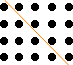
\includegraphics[width=0.1\textwidth]{sumall}
            \end{center}
  \end{parts}
  \question Justify observations 1 and 2 by counting cleverly.
  \question Give another proof for observation 5 by expanding $ (1 + 1)^n $ using the binomial theorem.
  \question Prove that, if we alternately add $ +$'s and $ -$'s between the members of each row of Pascal's triangle,
            then the resulting sum is zero. For example, $ 1 - 4 + 6 - 4 + 1 = 0 $. (Hint: $(1 - 1)^n = 0$.) Rephrase
            this in terms of binomial coefficients.
  \question A company once had a ``matching picture'' contest in which the object was to match the pictures of four
            celebrities with their baby pictures. Contestents were able to enter as many times as they wished, and
            the first prize was \$10,000.
    \begin{parts}
      \part How many different entries would you need to send in to be sure of having all four pictures matched correctly?
      \part Does it seem reasonable to think that you would win \$10,000 if you sent in an entry with all the pictures
            correctly matched?
    \end{parts}
  \question Let us calculate the number of ways there are to pick a team of seven out of a pool of twenty people, such that one
            of the members of the team is captain.
    \begin{parts}
      \part We can do this two ways; calculate both counts, and check they agree.
        \begin{subparts}
          \subpart Pick one captain out of twenty, and then six remaining players out of the 19 left.
          \subpart Pick seven players out of twenty, and then one captain out of the seven.
        \end{subparts}
      \part Prove the following generalisation in two different ways:
            \begin{displaymath}
              \binom{n}{b} \binom{n - b}{c} = \binom{n}{b + c} \binom{b + c}{b}
            \end{displaymath}
        \begin{subparts}
          \subpart As in (a), double-count the number of ways to pick a team of $ b + c $ players from $ n $, where $ b $ players are `special'.
          \subpart Algebraically, with the factorial definition of binomial coefficients.
        \end{subparts}
      \part Notice that the actual quantity in part (b)i is the number ways of picking \emph{three} subsets, of size $ x $, $ y $, and $ z $,
            from a set of $ n $, and the subsets \emph{partition} the set: use up all the elements without overcounting, so $ x + y + z = n $.
        \begin{subparts}
          \subpart Show that the number of ways to partition a set of size $ n $ using $ m $ smaller subsets, with sizes $ r_1, r_2, ..., r_m $,
                   is given by the \emph{multinomial coefficient}
                   \begin{displaymath}
                     \left\{\begin{array}{c}n\\r_1,r_2,\dots,r_m\end{array}\right\} = \frac{n!}{r_1! r_2! \cdots r_m!}.
                   \end{displaymath}
                   Hint: order $ n $, then chop off the first $ r_1 $ elements, then the next $ r_2 $ elements, and so on, taking account of ordering.
          \subpart Show that the binomial coefficients are special cases of the multinomial coefficients, but that
                   \begin{displaymath}
                     \binom{n}{r} \neq \left\{\begin{array}{c}n\\r\end{array}\right\}
                   \end{displaymath}
                   in general (hence why I use different brackets).
        \end{subparts}
    \end{parts}
  \question We have defined the number $ e $ to be $ \lim_n \left(1 + \frac{1}{n}\right)^n $.
    \begin{parts}
      \part Show that the $ i$th term in the expansion of $ \left(1 + \frac{1}{n}\right)^n $ for finite $ n $ is given by
            \begin{displaymath}
              \frac{n!}{(n - i!)i!n^i}.
            \end{displaymath}
      \part Suppose we hold $ i $ fixed, and send $ n $ off to infinity. Show that
            \begin{displaymath}
              \frac{n!}{(n - i)!} = n(n-1)(n-2)\cdots (n - i + i)
            \end{displaymath}
            for all $ i $, and conclude that
            \begin{displaymath}
              \frac{n!}{(n - i)! n^i}
            \end{displaymath}
            tends towards 1. (Hint: as $ n $ tends to infinity, but $ x $ remains finite, $ n - x \approx n $.)
      \part Hence, by expanding $ \left(1 + \frac{1}{n}\right)^n $ using the binomial theorem, show that
            \begin{displaymath}
              e = \lim_n \left(1 + \frac{1}{n}\right)^n = \frac{1}{0!} + \frac{1}{1!} + \frac{1}{2!} + \frac{1}{3!} + \cdots + \frac{1}{i!} + \cdots,
            \end{displaymath}
            and check that the two values roughly agree for $ n = 10 $.
    \end{parts}
\end{questions}

\end{document}
